\documentclass{article}

% if you need to pass options to natbib, use, e.g.:
%     \PassOptionsToPackage{numbers, compress}{natbib}
% before loading neurips_2021

% ready for submission
% \usepackage{neurips_2021}

% to compile a preprint version, e.g., for submission to arXiv, add add the
% [preprint] option:
    \usepackage[preprint]{neurips_2021}

% to compile a camera-ready version, add the [final] option, e.g.:
%     \usepackage[final]{neurips_2021}

% to avoid loading the natbib package, add option nonatbib:
%    \usepackage[nonatbib]{neurips_2021}

\usepackage[utf8]{inputenc} % allow utf-8 input
\usepackage[T1]{fontenc}    % use 8-bit T1 fonts
\usepackage{hyperref}       % hyperlinks
\usepackage{url}            % simple URL typesetting
\usepackage{booktabs}       % professional-quality tables
\usepackage{amsfonts}       % blackboard math symbols
\usepackage{nicefrac}       % compact symbols for 1/2, etc.
\usepackage{microtype}      % microtypography
\usepackage{xcolor}         % colors
\usepackage{graphicx}
\usepackage{float}
\usepackage{hyperref}
\usepackage{mathtools}
\usepackage{neuralnetwork}
% \addbibresource{sample.bib}
% \usepackage{biblatex}
\usepackage{tikz}
% \usetikzlibrary{positioning}

\title{CSE 151B Project Final Report}

% The \author macro works with any number of authors. There are two commands
% used to separate the names and addresses of multiple authors: \And and \AND.
%
% Using \And between authors leaves it to LaTeX to determine where to break the
% lines. Using \AND forces a line break at that point. So, if LaTeX puts 3 of 4
% authors names on the first line, and the last on the second line, try using
% \AND instead of \And before the third author name.

\author{%
  Alexander Friend \\
  \texttt{apfriend@ucsd.edu} \\
}

\begin{document}
  \maketitle
  \section{Task Description and Background}
    \subsection{Problem A [0.5 points]}        
      \textbf{Describe in your own words what the deep learning task is and
      why it is important. Provide some real-world examples where solving this task can have
      great impact on our daily life and the society.}

      The task for this Kaggle competition is to predict the positions of 60 individual 
      vehicles 3 seconds into the future, given an initial 2 second observation of vehicle positions and velocities, as
      well as data on relative lane positions. This is 
      an important task as autonomous vehicles (AV) are being increasingly rolled out to the public,
      and are expected to become the future standard of automobile transportation. In order 
      for this future to be realized however, AV's must be able to predict future movement and positions
      of objects in their visinity with high accuracy in order for AV's to be safer than human drivers.
    
    \subsection{Problem B [0.5 points]}
      \textbf{Use \href{https://scholar.google.com/}{Google Scholar} or other internet resources to research on
      this task. What type of methods have been examined before? Include some references and
      discuss their ideas in a few sentences. You can use 
      \href{https://www.overleaf.com/learn/latex/Bibliography_management_with_bibtex}{Bibtex} 
      to manage your bibliography.}

    \subsection{Problem C [1 points]}
      \textbf{Define the input and output in mathematical language and formulate your prediction task. 
      From the abstraction, do you think your model can potentially
      solve other tasks beyond this project? If so, list some examples and explain your rationale.}
              
      For this predition task, I will be taking in data on input and output positions, velocities, for $60$ cars in 
      a specific \emph{scene}, with lane information for each respective \emph{scene}. Each one of thes \emph{scenes}
      is a data point to be used to predict the output position of the 60 cars.

      My goal is to predict the positions of a specific car for 3 seconds into the future, in $\frac{1}{10}$ second intervals,
      using a prior $1.9$ seconds of data (also in $\frac{1}{10}$ second intervals).

      Since this prediction task relies on positional and velocity data, it can be generalized to any task that requires
      prediction of positions using prior positions, velocities, and lane information. In prediction models that do not use the 
      lane information, this task can be further abstracted to predicting future positions, using prior positions and velocities.

      This means that such a predictor may be able to be generalized to predict the future position of any moving object, using its
      prior positions and velocities.
        
  \section{Exploratory Data Analysis}
    \textbf{Perform exploratory data analysis and report your findings with texts/tables/figures. If
    you include more exploratory analysis beyond the listed questions that provides insights
    into the data, you will receive bonus points.}

    

    \subsection{Problem A [0.5 points]}
      \textbf{Run the provided Jupyter notebook for loading the data. Describe the details of this dataset. Your description
      should answer the following questions:}

      \begin{itemize}
        \item \textbf{what is the train/test data size?}
        \item \textbf{how many dimensions of inputs/outputs in the raw data?}
        \item \textbf{what are the meanings of these input/output dimensions?}
        \item \textbf{what does one data sample looks like?}
      \end{itemize}

      Our data is split into two sets, a training set and test set, title \texttt{new\_train} and 
      \texttt{new\_val\_in}, respectively. The training dataset contains the following fields: 
      
      \begin{itemize}            
          \item {\fontfamily{qcr}\selectfont p\_in} - the (x,y) position input in the first two seconds (19 time steps)
          \item {\fontfamily{qcr}\selectfont v\_in} - the (x,y) velocity input in the first two seconds (19 time steps)
          \item {\fontfamily{qcr}\selectfont p\_out} - the (x,y) position output in the next three seconds (30 time steps)
          \item {\fontfamily{qcr}\selectfont v\_out} - the (x,y) velocity output in the next three seconds (30 time steps)
          \item {\fontfamily{qcr}\selectfont track\_id} - the track\_id for each vehicle in the output sequence (30 time steps). This 
                is a unique value for each object in the \emph{scene}, not every object in the whole dataset.
          \item {\fontfamily{qcr}\selectfont scene\_idx} - the id of a specific scene, i.e each one of the $205,944$ and $3,200$  
                training and validation datasets.
          \item {\fontfamily{qcr}\selectfont agent\_id} - track id for an agent (car), of which the task is to predict its future position. 
          \item {\fontfamily{qcr}\selectfont car\_mask} - boolean index for the real car, which matches the first dimension of its 
               corresponding \texttt{track\_id}, \texttt{p\_in}, \texttt{p\_out}, \texttt{v\_in}, and \texttt{v\_out}. 
          \item {\fontfamily{qcr}\selectfont lane} - (x,y,z) for centerline nodes in this scene (z position is always $0$). 
                There may be more than one lane in a scene, however this amount may vary from scene to scene.
          \item {\fontfamily{qcr}\selectfont lane\_norm} - (x,y,z) the direction of each lane node (z position is always $0$)
      \end{itemize}

      The validation dataset contains the same fields as the training set, except it is lacking the \texttt{p\_out} and
      \texttt{v\_out} fields, as these are the fields to be predicted. 
      
      Using these datasets, our all possible input data will be the the positions (\texttt{p\_in}), velocities 
      (\texttt{v\_in}). Each input position and velocity data is of the shape $60 \times 19 \times 2$, and each output
      position and velocity data is of the shape $60 \times 30 \times 2$. The dimension represents the $60$ agents (AV's)
      in the datapoints scene. The second dimension represents the number of times each agents' position and velocity is tracked.
      $19$ times for $1.9$ seconds for the input data, and $30$ times for $3$ seconds for the outputs. Finally the third dimension
      represents the respective $x$ and $y$ positiona and velocity vectors for each agent.
      
      The ID's of each of the $60$ vehicles (\texttt{track\_id}) in validation set, which will be represented by a $60 \times 30 \times 1$ tensor.
      The first dimension is to represent each individual agent in the vehicle, and each of the $30$ values in the second dimension
      is identical. 
      
      Furthermore lane information will include the position of the center of the lanes (\texttt{lane\_id}), 
      which is of dimensions $K \times 3$, where $K$ is the number of lanes in
      a scene, and each one of the $3$ values represents an $x,y,z$ coordinate. The $z$ coordinates are always $0$, while the $x,y$
      data can be either negative as well as positive, where negative values indicate that the center of a respective lane
      is near the edge of the coordinate system. Additionally the direction of each lane 
      (\texttt{lane\_norm}) is of the dimension $K \times 3$, where $K$ is the number of lanes in
      a scene, and each one of the $3$ values represents an $x,y,z$ coordinate. Similarly to the \texttt{lane\_id} data, each 
      \texttt{lane\_norm} has values of $0$ for each $z$ coordinate, however the $x,y$ data can be either positive or negative, 
      representing which direction relative to the lane center that the lane is pointing.

      The training data set contains $205,944$ training scenes, and the validation set contains $3,000$ scenes. 

      Not all of this data may be extremely useful however, as incorporating the lane information will lead to an increase in complexity
      of any prediction model, which may not be necessary to produce an accurate prediction. The most important information to predict
      the future positions of an AV will the the input and output positions and velocities, as well as the \texttt{agent\_id} which is 
      necessary to identify the car wished to be tracked. The lane information, may still be useful in more complex models in order to 
      account for changes in direction, which may be difficult to impossible to achieve using only prior positions and velocities.

      

    \subsection{Problem B [0.5 points]}
      \textbf{Perform statistical analysis to understand the properties of the data. Your analysis should at least
      answer the following questions.}
      
      \begin{itemize}
        \item \textbf{what is the distribution of input positions/velocity (magnitude) for all agents}
        \item \textbf{what is the distribution of output positions/velocity (magnitude) for all agents}
        \item \textbf{what is the distribution of positions/velocity (magnitude) for the target agent}
      \end{itemize}

      \begin{table}[h!]
        \centering
        \begin{tabular}{|| c | c c c c||} 
        \hline
        Statistic & $x$-Position & $y$-Position & $x$-Velocity & $y$-Velocity\\ [0.5ex] 
        \hline\hline
        count &	2.280000e+06 & 2.280000e+06 & 2.280000e+06 & 2.280000e+06\\
        mean & 2.108387e+02 & 3.245734e+02 & 3.604328e-02 & -1.889331e-02\\
        std & 7.032012e+02 & 8.485306e+02 & 1.749104e+00 & 2.185653e+00\\
        min & 0.000000e+00 & 0.000000e+00 & -1.144689e+02 & -1.688118e+02\\
        25 & 0.000000e+00 & 0.000000e+00 & 0.000000e+00 & 0.000000e+00\\
        50 & 0.000000e+00 & 0.000000e+00 & 0.000000e+00 & 0.000000e+00\\
        75 & 0.000000e+00 & 0.000000e+00 & 0.000000e+00 & 0.000000e+00\\
        max & 4.735943e+03 & 4.092156e+03 & 7.909621e+01 & 1.461265e+02\\
        \hline
        \end{tabular}
        \caption{Table of input positions and velocities of sample}
        \label{table:1}
    \end{table}
    
    \begin{table}[h!]
        \centering
        \begin{tabular}{|| c | c c c c||} 
        \hline
        Statistic & $x$-Position & $y$-Position & $x$-Velocity & $y$-Velocity\\ [0.5ex] 
        \hline\hline
        count & 3.600000e+06 & 3.600000e+06 & 3.600000e+06 & 3.600000e+06\\
        mean & 2.109253e+02 & 3.245277e+02 & 3.481067e-02 & -1.777745e-02\\
        std & 7.034579e+02 & 8.483126e+02 & 1.797118e+00 & 2.223628e+00\\
        min & 0.000000e+00 & 0.000000e+00  & 1.008539e+02 & -1.215008e+02\\
        25 & 	0.000000e+00 & 0.000000e+00 & 0.000000e+00 & 0.000000e+00\\
        50 & 	0.000000e+00 & 0.000000e+00 & 0.000000e+00 & 0.000000e+00\\
        75 & 	0.000000e+00 & 0.000000e+00 & 0.000000e+00 & 0.000000e+00\\
        max & 4.736574e+03 & 4.092117e+03 & 8.774132e+01 & 1.484342e+02\\
        \hline
        \end{tabular}
        \caption{Table of Output positions and velocities of sample}
        \label{table:2}
    \end{table}

    \begin{figure}[H]
        \centering
        \includegraphics[height=6cm]{figures/sample-in-position-hist.pdf}%
        \caption{Histogram of the X and Y input positions from a subsample of 2000 training files}%
        \label{fig:1}
    \end{figure}        
            
    \begin{figure}[H]
        \centering
        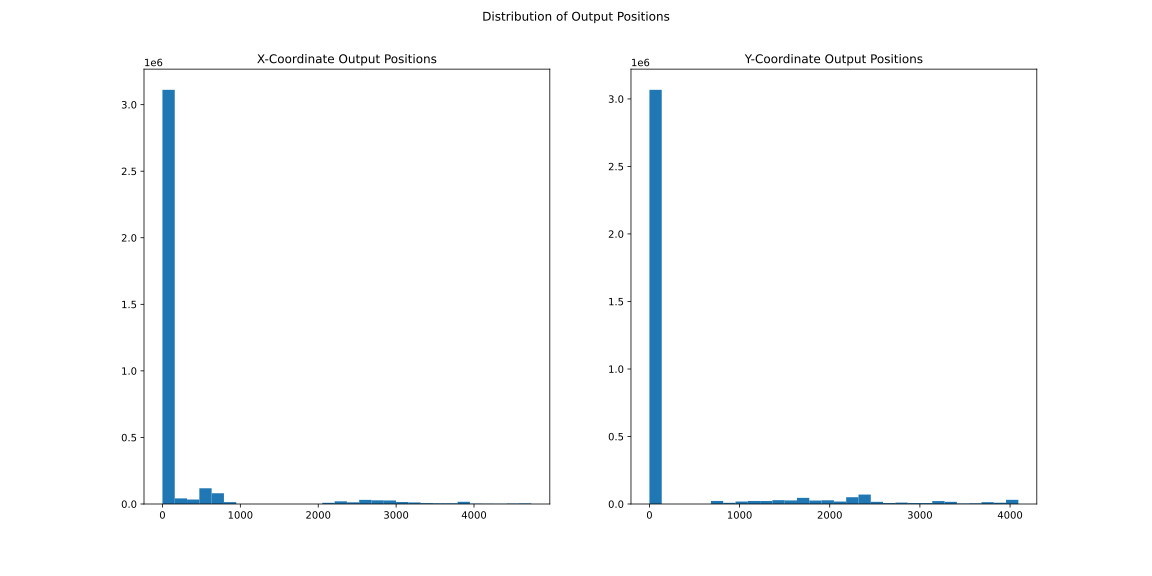
\includegraphics[height=6cm]{figures/sample-out-position-hist.pdf}%
        \caption{Histogram of the X and Y output positions from a subsample of 2000 training files}%
        \label{fig:2}
    \end{figure}

    Analyzing these inputs we find that the vast majority of $(x,y)$ input and output positions are at position $0$, as seen in 
    \autoref{fig:1}, \autoref{fig:2}, and \autoref{table:1} above. Interestingly, the $x$-positions seem to be 
    more closely clustered around $0$, while the $y$-positions 
    have more variance, meaning that most cars are moving mostly in the $y$-dimension, with less overall travel in the $x$-dimension. This
    trend carries through the beginnning and end of the scene (the input and output data).
    
    Looking at only the magnitudes of velocities shows the same trend, with the vast majority of velocities being
    0, however there is also slightly more variance in the distribution of velocties in the $y$-dimension compared to 
    the $x$-dimension.
    
    \subsection{Problem C [1 points]}
      \textbf{Process the data to prepare for the prediction task. Describe the
      steps that you have taken to process the data. Your description should at least answer the
      following questions.}
      
      \begin{itemize}
        \item \textbf{Did you use any feature engineering? If yes, how did you design your features?
        Explain your rationale.}
        \item \textbf{How did you normalize your data? Why did you choose this normalization scheme?}
        \item \textbf{Did you use the lane information provided in the dataset. If yes, how did you
        exploit this information.}
      \end{itemize}

      In order to prepare my data, I used batch normalization for each input $(x,y)$ position and velocity vectors.
      This was in order to ensure that my models would predict the future positions based on relative positions and velocities
      in each respective scene, rather than the absolute position and velocity. This is based on the idea that actual people driving
      move in react based on relative positions and speeds of objects in their area, not based on absolute geospatial coordinates.

      At this point I have not used any lane information, as my models are still on the simpler side due, however this is something
      I wish to imncorporate in future work. Using this information in a model would require normalization relative to the 
      center of each lane as well. For more detail see section \ref{future-work}.

  \section{Deep Learning Model}
    \subsection{Problem A [1 Points]}
      \textbf{Describe the deep learning pipeline for your prediction task and
      answer the following questions.}

      \begin{itemize}
        \item \textbf{What are the input/output that you end up using for prediction after preprocessing?}
        \item \textbf{What is your loss function? If you have multiple alternatives, discuss your ideas
        and observations.}
        \item \textbf{How did you decide on the deep learning model? Explain the rationale given the
        input/output.}
      \end{itemize}

      I ended up using the positions (\texttt{p\_in}) and velocities (\texttt{v\_in}) as a single tensor as input data for my models, with 
      the models predicting the output positions (\texttt{p\_out}) and velocities (\texttt{v\_out}) as a single tensor. 
      Only the output position data ended up being used for this specific prediction task however. 
      
      As a loss function I used both mean squared error (MSE), and root mean square error (RMSE). I ended up using RMSE as my 
      final loss function however, as this is the 
      same loss being used by the Kaggle competition leaderboard. Using RMSE as a loss function allowed me to better judge how my 
      models were performing relative to others in the competition.

      I used single layer and $2$ multilayer regression neural networks, as well as a Long Short-Term Memory (LSTM) neural network as models for my prediction task.
      The multilayer regression model used $3$ linear layers. I chose the single and multilayer regression models as they are simple models
      to start out with, making developing better models easier to do. They also are well suited for predicting future position as an equation of 
      starting position and time. An LSTM approach was chosen since a RNN architecture allows for using previous predicted sequences
      to predict future sequences, which is useful for predicting multiple positions in a time series. I chose a LSTM specifically as it 
      is able to remember previous hidden states, which alleviates the vanishing gradient problem often seen in RNN architectures.

    \subsection{Problem B [1 Points]}        
      \textbf{Describe all the models you have tried to make predictions. You
      should always start with simple models (such as Linear Regression) and gradually 
      increase the complexity of your model.}
 
      \begin{itemize}
        \item \textbf{Use an itemized list to briefly summarize each of the models, their architecture, and
        parameters, and provide the correct reference if possible.}
        \item \textbf{If you end up designing your own model architecture, include a picture/sketch of
        your model architecture. Explain why you choose such a model.}
        \item \textbf{Describe different regularization techniques that you have used such as dropout
        and max-pooling in your model.}
      \end{itemize}

      \textbf{You can also use mathematical equations to explain your prediction logic.}]

      In addition to the single layer linear regression neural network, $2$ multiple layer nerual network, and LSTM models, I used a 
      non deep-learning model based in simple Newtonian physics, using average velocity and a starting position to predict future 
      positions.

      \begin{enumerate}
        \item "Physics Model" (1) 
        \label{itm:1}
        \begin{enumerate}
          \item This model uses kinematic equations from physics to predict future position. Specifically it computes the average
                input velocity of each agent in a scene and uses the final input position coordinate to predict the position of each 
                future time step.
          \item It can be summarized by the equations: 
          $$\vec{r}_{out}^{(t)} \approx \vec{r}_{in}^{(19)} + \left( \frac{1}{N}\sum_{i=1}^{N}{\vec{v}^{(i)}} \right) \cdot \Delta t$$
          \begin{enumerate}
            \item Where $\vec{r}^{(19)}_{in} \in \big( \begin{smallmatrix}
                                        x\\
                                        y\\
                                      \end{smallmatrix} \big)$
                  is the position vector in $2d$ space at the $19$th time step in the input data.
            \item $\vec{r}^{(t)}_{out} \in \big( \begin{smallmatrix}
              x\\
              y\\
            \end{smallmatrix} \big)$ is the position  vector in $2d$ space at the $t$th time step in the output data.
            \item $\vec{v}^{(i)} \in 
              \big( \begin{smallmatrix}
                v^{(i)}_{x}\\
                v^{(i)}_{y}
              \end{smallmatrix} \big)$ is the velocity vector in $2d$ space at input time step $i$
            \item $\Delta t$ represents each consecutive time step for the prediction task, which is up to 3 seconds 
                  predicted at a rate of $\frac{1}{10}$ per second. $\Delta t \in [1,30]$
            \item $N$ corresponds to each the number of time step in the training data, in this case $N=19$ for each position
                  and velocity vector measured for $1.9$ seconds at a rate of $\frac{1}{10}$ per second
          \end{enumerate}
          % \end{enumerate}
        \end{enumerate}

        \item Single Layer Linear Regression Neural Network (2) 
        \label{itm:2}
        \begin{enumerate}
          \item A single layer PyTorch linear regression model, which takes the input position and velocity tensors and predicts
                for 19 time steps and predicts the output position and velocity tensors.
          \item The input layer is of shape $\left(1, 60 \times 19 \times 4\right)$, and the output layer is of shape 
                $\left(1, 60 \times 30 \times 4\right)$
          \item Input is a tensor of shape $\left( \mathrm{batch\ size}, 60, 19, 4 \right)$ reshaped
                to a tensor of dimensions $\left( \mathrm{batch\ size}, 60 \times 19 \times 4 \right)$ when fed to the model
          \begin{enumerate}
                \item $\mathrm{batch\ size}$ is the number of scenes in a mini-batch duriung each training iteration in an epoch.
                \item The second dimension of this tensor represents the $60$ individual agents tracked in each respective scene 
                      in a mini-batch 
                \item The third dimension represents the $19$ time steps measured in the $1.9$ second period.
                \item The first $2$ elements of the $4th$ dimension of this tensor are the position coordinates in $2d$ space, and the last $2$ elements of the 
                tensor's $4th$ dimension are the velocity coordinates in $2d$ space for each respective agent in the mini-batch.
          \end{enumerate}
          \item Output is a tensor of shape $\left( \mathrm{batch\ size}, 60 \times 30 \times 4 \right)$ to a tensor of 
                shape $\left( \mathrm{batch\ size}, 60, 30, 4 \right)$.
          \begin{enumerate}
            \item $\mathrm{batch\ size}$ is the number of scenes in a mini-batch duriung each training iteration in an epoch.
            \item The second dimension of this tensor represents the $60$ individual agents tracked in each respective scene 
                  in a mini-batch 
            \item The third dimension represents the $30$ time steps measured in the $3$ second period.
            \item The first $2$ elements of the $4th$ dimension of this tensor are the position coordinates in $2d$ space, and the last $2$ elements of the 
            tensor's $4th$ dimension are the velocity coordinates in $2d$ space for each respective agent in the mini-batch.
          \end{enumerate}
          \item Position predictions are made by selecting the first two elements from the $4th$ dimension of each tensor, where the 
                \texttt{agent\_id} in the corresponding $2nd$ dimension of each tensor matches the desired \texttt{agent\_id}'s from the 
                validation dataset
          \label{itm:6}
          \item See \autoref{fig:3} in \autoref{sec:appendix} for a visualization of this model 
        \end{enumerate}

        \item Multiple Layer Linear Regression Neural Network (3) 
        \label{itm:3}
        \begin{enumerate}
          \item A PyTorch neural network with linear input and output layers, and a hidden activation function layer,
                 which takes the input position and velocity tensors and predicts
                for 19 time steps and predicts the output position and velocity tensors.
          \item The output and input layers are the same shape as of model \ref{itm:2}
          \item The single hidden layer uses the \emph{ReLU} activation function, which was chosen as this function is generally the best performing
                activation function for neural networks, and it allows for non positive neurons in the hidden layer are activated, since these
                are the only non-zero outputs from the \emph{ReLU} activation function.\hyperref[bibliography]{[1]}
          \item The hidden layer is of dimension 1024.
          \item Input and Output tensors are the same shape as model \ref{itm:1}
          \item Position Predictions are selected in the same manner as model \ref{itm:1}
          \item See \autoref{fig:4} in \autoref{sec:appendix} for a visualization of this model 
        \end{enumerate}

        \item Multiple Layer Linear Regression Neural Network (4) 
        \label{itm:4}
        \begin{enumerate}
          \item A PyTorch neural network with linear input and output layers, and 3 hidden activation function layers, as well 
                as 3 hidden linear layers, which takes the input position and velocity tensors and predicts
                for 19 time steps and predicts the output position and velocity tensors.
          \item The output and input layers are the same shape as of model \ref{itm:2}
          \item The hidden layers consist of an \emph{ReLU} activation layer of dimension 2048, fed to a linear layer which takes in  
          \item The activation function between the first 3 layers is \emph{ReLU}, the motivation behind this choice is the same as explained 
                for model \ref{itm:3}. The final hidden
          \item The hidden layer is of dimension 1024.
          \item Input and Output tensors are the same shape as model \ref{itm:1}
          \item Position Predictions are selected in the same manner as model \ref{itm:1}
          \item See \autoref{fig:5} in \autoref{sec:appendix} for a visualization of this model 
        \end{enumerate}
        \item Long Short-Term Memory (LSTM) and CNN Model (5) 
        \label{itm:5}
        \begin{enumerate}
          \item PyTorch LSTM layers with a final convolutional layer to map to the output tensor.
          \item The LSTM layers consist of an input layer of shape $\left( 60 \times 4, 1 \right)$ with 2 hidden layers of shape 
                $\left( 2048 \times 4, 1 \right)$
          \item The Convolutional layer has $240$ channels and takes in the inputs of the hidden layer,
                of shape $\left( 2048 \times 4, 1 \right)$, and returns them to an output layer of shape $\left( 60 \times 4, 1 \right)$
          \item Position Predictions are selected in the same manner as model \ref{itm:1}
        \end{enumerate}
      \end{enumerate}

  \section{Experimental Design}
    \subsection{Problem A [1 points]}
      \textbf{Describe how you set up the training and testing design for deep learning. Answer the following questions:}

      \begin{itemize}
        \item \textbf{What computational platform/GPU did you use for training/testing?}
        \item \textbf{How did you split your training and validation set?}
        \item \textbf{What is your optimizer? How did you tune your learning rate, learning rate decay,
        momentum and other parameters?}
        \item \textbf{How did you make multistep (30 step) prediction for each target agent?}
        \item \textbf{How many epoch did you use? What is your batch-size? How long does it take to
        train your model for one epoch (going through the entire training data set once)?}
      \end{itemize}

    \textbf{Explain why you made these design choices. Was it motivated by your past experience?
    Or was it due to the limitation from your computational platform? You are welcome to
    use screenshots or provide code snippets to explain your design.}

    The platform I am currently working in is my local machine running Ubuntu $20.04$ with a $4$-core $4$-thread Intel i$7$-$7600$k CPU 
    running at $4.2$ GHz, a GTX $1070$ GPU with a max clock speed of $1721$ MHz and $8$ GB of GDDR5 memory, and $32$ GB of $3000$ MHz DDR4 memory.
    Since the start of this project, I have upgraded my local machine from $16$ GB to $32$ GB of RAM.

    I used all $202,944$ training data sets, with the remaining $3,000$ training data sets set aside as a test set. This test set was randomly sampled
    to be the same size as the batch size for each model I implemented, with the exception of the \hyperref{"physics model"}{itm:1}. Since this model 
    was not a deep learning model and did not have any requirements for batch size, the entire test set of $3,000$ scenes was used to test the loss
    of this model.

    I used Adam with a learning rate of $0.3$ as my optimizer since it implements an updating momentum, based on the gradient, 
    meaning that it will converge more quickly to an estimate of the gradient. Additionally,
    Adam utilizes a mini-batch approach to approximating the gradient, similar to Stochastic Gradient Descent (SGD), which allows for better 
    parallelization, and generalization, as well as the added benefit of using less memory, potentially increasing computational performance.

    For my \hyperref{physics based model}{itm:1} using average velocity, I predicted each time step by multiplying the average velocity
    from the $N=19$ time steps in the input data by the amount
    of time elapsed since the last tracked input, and then added this to the last tracked position. For example the first and last 
    time steps at $t=0.1$ and $t=3$ seconds after the last input data, respectively: 
    \begin{align*}
      \vec{r}_{out}^{(1)} \approx& \vec{r}_{in}^{(19)} + \left( \frac{1}{N}\sum_{i=1}^{N}{\vec{v}_{i}} \right) \cdot 0.1\\
      \vec{r}_{out}^{(30)} \approx& \vec{r}_{in}^{(19)} + \left( \frac{1}{N}\sum_{i=1}^{N}{\vec{v}_{i}} \right) \cdot 3
    \end{align*}

    The deep learning models would each produce outputs predicting the positions and velocities for each of the $30$ times steps into 
    the future. Extracting the predictions for these was as simple as just extracting the position elements from the outputted tensor.

    Both models outputted tensors predicting the positions for all agents in a scene. So the element corresponding to the desired agents in the 
    validation set were selected, as described further in \hyperref[itm:6]{Section 3.2.2.e}

    \hyperref[itm:2]{Model 2} and \hyperref[itm:3]{model 3} were trained for $1$, $5$, $10$ and $20$ epochs, with batch sizes of $128$, $64$, $32$, 
    and $16$. \hyperref[itm:3]{Model 3} was also trained with batch sizes of  $128$, $64$, $32$, and $16$, however it was only trained for $1$, $5$, 
    and $10$ epochs as the loss of that model did not decrease after any more training. \hyperref[itm:5]{Model 5} was only trained for $5$ epochs with 
    a batch size of $128$ due to a lack of time (see Section \ref{future-work} for more details on future plans).

  \section{Experiment Results}
    \subsection{Problem A [1 points]}
      \textbf{Select a few representative models of yours and report the following results by comparing different models.} 
      
      \begin{itemize}
        \item \textbf{Use a table to compare the performances of different model designs. What conclusions can you draw from this table.}
        \item \textbf{Provide an estimate of training time (in flops or minutes) for different models. What
        did you do to improve the training speed?}
        \item \textbf{Count and report the number of parameters in different models.}
      \end{itemize}

    \subsection{Problem B [1 points]}
      \textbf{Play with different designs of your model and experiments and report the following for your best-performing design:} 
      
      \begin{itemize}
        \item \textbf{Visualize the training/validation loss (RMSE) value over training steps (You should
        expect to see an exponential decay).}
        \item \textbf{Randomly sample a few training samples after the training has finished. Visualize
        the ground truth and your predictions.}
        \item \textbf{Your current ranking on the leaderboard and your final test RMSE.}
      \end{itemize}
    
  \section{Discussion and Future Work}\label{future-work}
    \subsection{Problem A [1 points]}
      \textbf{Analyze the results and identify the lessons/issues that you have learned so far. Briefly answering the following questions.} 
      
      \begin{itemize}
        \item \textbf{What do you think is the most effective feature engineering strategy?}
        \item \textbf{What techniques (data visualization/model design/hyper-parameter tuning) did
        you find most helpful in improving your score?}
        \item \textbf{What was your biggest bottlenect in this project?}
        \item \textbf{How would you advise a deep learning beginner in terms of designing deep learn-
        ing models for similar prediction tasks.}
        \item \textbf{If you had more resources, what other ideas would you like to explore?}
      \end{itemize}      

  \appendix

   \section{Appendix}
      \label{sec:appendix}

      \begin{figure}[H]
        \centering
        \includegraphics[height=6cm]{figures/single-layer-net.png}%
        \caption{Diagram of single layer model \ref{itm:2}}%
        \label{fig:3}
      \end{figure}

      \begin{figure}[H]
        \centering
        \includegraphics[height=6cm]{figures/multi-layer-net1.png}%
        \caption{Diagram of single layer model \ref{itm:3}}%
        \label{fig:4}
      \end{figure}

      \begin{figure}[H]
        \centering
        \includegraphics[height=6cm]{figures/multi-layer-net2.png}%
        \caption{Diagram of single layer model \ref{itm:4}}%
        \label{fig:5}
      \end{figure}

  \url{https://github.com/apfriend/cse151b-kaggle.git}

  \section*{References}
  \label{bibliography}
    \medskip{
      \small
      
      [1] Siddharth Sharma\ \&Simone Sharma\ \&Anidhya Athaiya(2020) ACTIVATION FUNCTIONS IN NEURAL
      NETWORKS. In G.\ Tesauro, D.S.\ Touretzky and T.K.\ Leen
      (eds.), {\it International Journal of Engineering Applied Sciences and Technology}, Vol. 4, Issue 12,
      pp.\ 310--316. [Online]. Available: \url{https://www.ijeast.com/papers/310-316,Tesma412,IJEAST.pdf}
      
      [2] Bower, J.M.\ \& Beeman, D.\ (1995) {\it The Book of GENESIS: Exploring
        Realistic Neural Models with the GEneral NEural SImulation System.}  New York:
      TELOS/Springer--Verlag.
      
      [3] Hasselmo, M.E., Schnell, E.\ \& Barkai, E.\ (1995) Dynamics of learning and
      recall at excitatory recurrent synapses and cholinergic modulation in rat
      hippocampal region CA3. {\it Journal of Neuroscience} {\bf 15}(7):5249-5262.
    }

\end{document}